\documentclass{article}
\usepackage[utf8]{inputenc}
\usepackage{graphicx}
\usepackage{tikz}

\usepackage{amsmath, amsthm, amssymb}

\usepackage{tkz-euclide}

\usepackage{gensymb}

\usetikzlibrary{calc}

\usepackage{multicol,multirow}

\title{Practicando en LATEX}
\author{javier argo}


\begin{document}

\tableofcontents
\listoffigures

\maketitle
\section{Introduction}

\begin{figure}[h]
    \centering
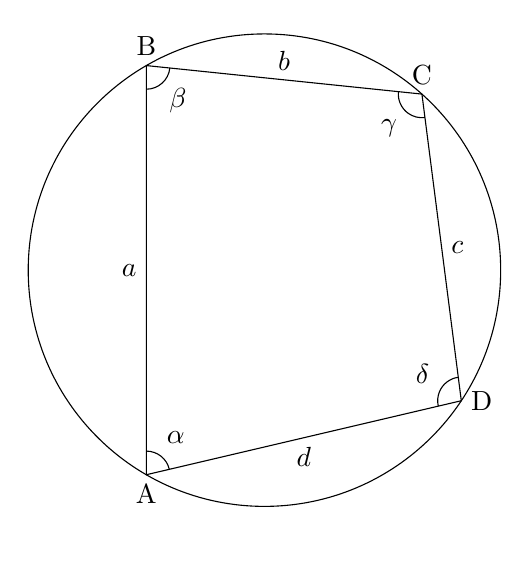
\begin{tikzpicture}
% círculo:
\draw (0,0) circle (3cm);
%cuadrilatero
\coordinate (A) at (-1.5,{-sqrt(27)/2});
\coordinate (B) at (-1.5,{sqrt(27)/2});
\coordinate (C) at (2, {sqrt(5)});
\coordinate (D) at (2.5,{-sqrt(11)/2});
\draw (A) -- (B) -- (C) -- (D) -- cycle;
\node[below] at(A) {A};
\node[above] at(B) {B};
\node[above] at(C) {C};
\node[right] at(D) {D};

\tkzMarkAngle[size=0.3cm](B,C,D);
\tkzMarkAngle[size=0.3cm](A,B,C);
\tkzMarkAngle[size=0.3cm](C,D,A);
\tkzMarkAngle[size=0.3cm](D,A,B);
\tkzLabelAngle[pos=-.6](B,A,D){$\alpha$}
\tkzLabelAngle[pos=.6](A,B,C){$\beta$}
\tkzLabelAngle[pos=.6](B,C,D){$\gamma$}
\tkzLabelAngle[pos=.6](C,D,A){$\delta$}
\tkzLabelSegment[left](A,B){$a$}
\tkzLabelSegment[above](B,C){$b$}
\tkzLabelSegment[right](C,D){$c$}
\tkzLabelSegment[below](D,A){$d$}

\end{tikzpicture}  
\caption{Cuadrilátero inscrito}
   
\end{figure}

Se cumple:
%formula
\[ \frac{\tan(\frac{1}{2}(\alpha-\beta))}{\tan(\frac{1}{2}(\alpha+\beta))} = \frac{(a-c)(b-d)}{(a+c)(b+d)} \]

\newpage
%*********************

% EJERCICIO
\section{Introduction}

\begin{figure}[h]
    \centering
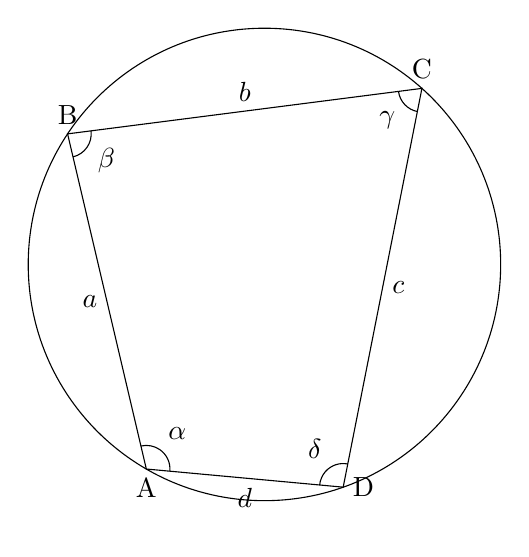
\begin{tikzpicture}
% círculo:
\draw (0,0) circle (3cm);
%cuadrilatero
\coordinate (A) at (-1.5,{-sqrt(27)/2});
\coordinate (B) at (-2.5,{sqrt(11)/2});
\coordinate (C) at (2, {sqrt(5)});
\coordinate (D) at (1,{-sqrt(8)});
\draw (A) -- (B) -- (C) -- (D) -- cycle;
\node[below] at(A) {A};
\node[above] at(B) {B};
\node[above] at(C) {C};
\node[right] at(D) {D};

\tkzMarkAngle[size=0.3cm](B,C,D);
\tkzMarkAngle[size=0.3cm](A,B,C);
\tkzMarkAngle[size=0.3cm](C,D,A);
\tkzMarkAngle[size=0.3cm](D,A,B);
\tkzLabelAngle[pos=-.6](B,A,D){$\alpha$}
\tkzLabelAngle[pos=.6](A,B,C){$\beta$}
\tkzLabelAngle[pos=.6](B,C,D){$\gamma$}
\tkzLabelAngle[pos=.6](C,D,A){$\delta$}
\tkzLabelSegment[left](A,B){$a$}
\tkzLabelSegment[above](B,C){$b$}
\tkzLabelSegment[right](C,D){$c$}
\tkzLabelSegment[below](D,A){$d$}

\end{tikzpicture}  
\caption{Cuadrilátero inscrito}
   
\end{figure}

Se cumple:
%formula
\[ \frac{ab+cd}{\sin(\alpha)}=\frac{ad+bc}{\sin(\beta)}=\frac{ab+cd}{\sin(\gamma)}=\frac{ad+bc}{\sin(\delta)} \]

\newpage
%*********************
% EJERCICIO
\section{Introduction}

\begin{figure}[h]
\centering
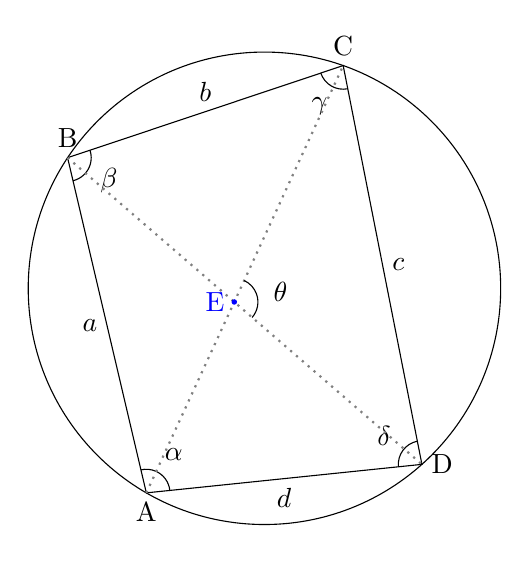
\begin{tikzpicture}
% círculo:
\draw (0,0) circle (3cm);
%cuadrilatero
\coordinate (A) at (-1.5,{-sqrt(27)/2});
\coordinate (B) at (-2.5,{sqrt(11)/2});
\coordinate (C) at (1,{sqrt(8)});
\coordinate (D) at (2, {-sqrt(5)});
\draw (A) -- (B) -- (C) -- (D) -- cycle;
\node[below] at(A) {A};
\node[above] at(B) {B};
\node[above] at(C) {C};
\node[right] at(D) {D};

\tkzMarkAngle[size=0.3cm](B,C,D);
\tkzMarkAngle[size=0.3cm](A,B,C);
\tkzMarkAngle[size=0.3cm](C,D,A);
\tkzMarkAngle[size=0.3cm](D,A,B);
\tkzLabelAngle[pos=-.6](B,A,D){$\alpha$}
\tkzLabelAngle[pos=.6](A,B,C){$\beta$}
\tkzLabelAngle[pos=.6](B,C,D){$\gamma$}
\tkzLabelAngle[pos=.6](C,D,A){$\delta$}
\tkzLabelSegment[left](A,B){$a$}
\tkzLabelSegment[above](B,C){$b$}
\tkzLabelSegment[right](C,D){$c$}
\tkzLabelSegment[below](D,A){$d$}

\draw[gray, dotted, thick] (B) -- (D);
\draw[gray, dotted, thick] (A) -- (C);

\coordinate (E) at (intersection of A--C and B--D);
 \fill[blue] (E) circle (1pt) node[ left]{E};
 {((C)+(A)+(D)+(B))}/2;
%\coordinate (E) at (-0.25,1); %({(C)+(A)-(D)-(B)})/2; \filldraw[black] (E) circle (1pt) node[ pos=.6]{E};
\tkzMarkAngle[size=0.3cm](D,E,C);
\tkzLabelAngle[pos=.6](D,E,C){$\theta$}

\end{tikzpicture}  
\caption{Cuadrilátero inscrito}
   
\end{figure}

Se cumple:
%formula
\[ \frac{\sin(\frac{\alpha+\beta}{2})}{\cos(\frac{\gamma-\delta}{2})} =\frac{a+c}{b+d}\cot(\frac{\theta}{2})\]


\newpage
%*********************
% EJERCICIO
\section{Teorema de Papillon}

\begin{figure}[h]
\centering
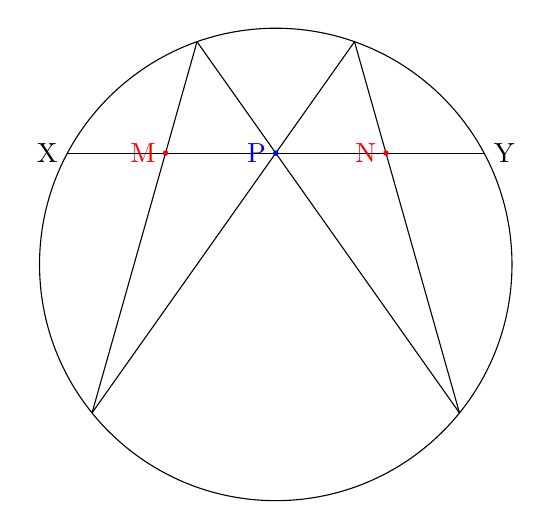
\begin{tikzpicture}
% círculo:
\draw (0,0) circle (3cm);
%recta
\coordinate (Y) at ({sqrt(7)},{sqrt(2)});
\coordinate (X) at ({-sqrt(7)},{sqrt(2)});
\draw (X) -- (Y);

%cuadrilatero
\coordinate (A) at ({-7/3},{(-sqrt(32))/3});
\coordinate (B) at (-1,{sqrt(8)});
\coordinate (C) at (1,{sqrt(8)});
\coordinate (D) at ({7/3},{(-sqrt(32))/3});
\draw (A) -- (C);
\draw (A) -- (B);
\draw (C) -- (D);
\draw (B) -- (D);
\node[left] at(X) {X};
\node[right] at(Y) {Y};

\coordinate (P) at (intersection of A--C and B--D);
 \fill[blue] (P) circle (1pt) node[ left]{P};
 
 \coordinate (M) at (intersection of A--B and X--Y);
 \fill[red] (M) circle (1pt) node[ left]{M};
 
  \coordinate (N) at (intersection of C--D and X--Y);
 \fill[red] (N) circle (1pt) node[ left]{N};

\end{tikzpicture}  
\caption{Cuadrilátero inscrito}
\end{figure}

Sea la circunferencia:\\ \\
Si $\overline{XP}=\overline{PY}$, entonces:
$$\overline{MP}=\overline{PN}$$
\newpage

%*********************
% EJERCICIO
\section{Teorema de Visscher}

\begin{figure}[h]
    \centering
\begin{tikzpicture}
%triangulo
\coordinate (A) at (-1,-2);
\coordinate (B) at (-3,5);
\coordinate (C) at (2,-2);
\coordinate (D) at (0,0);
\draw (A) -- (B) -- (C) -- cycle;
\node[below] at(A) {A};
\node[above] at(B) {B};
\node[right] at(C) {C};
\node[right] at(D) {D};
\draw[gray, dotted, thick] (B) -- (D);
\draw[gray, dotted, thick] (A) -- (D);
\draw[gray, dotted, thick] (C) -- (D);

\end{tikzpicture}  
\caption{Triángulo}
\end{figure}
Sea el $\triangle ABC$.  
Si $\overline{AC}< \overline{AB}<\overline{BC}$ y $P$ es un punto medio dentro de la región triangular.\\

Entonces:
\begin{equation}
    \overline{AD} + \overline{BD} + \overline{CD} < \overline{AB} + \overline{BC}
\end{equation}



\newpage
%*********************
%ejercicio suelto
\begin{figure}
    \centering
    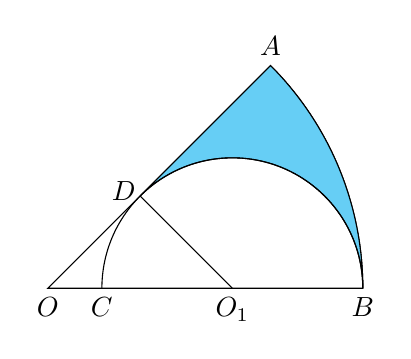
\begin{tikzpicture}
\draw (0,0) node [below]{$O$};

\draw (4,0) node [below]{$B$};
\draw (45:4) node [above]{$A$};
\draw (45:1.75) node [left]{$D$};
\draw (0:0.68629) node [below]{$C$};
\draw (0:2.343145) node [below]{$O_1$};
\draw (0:4) arc [start angle=0, end angle=45, radius=4] --(0,0) -- cycle ;

\draw (45:1.6568)--(2.3432,0);

\draw[fill=cyan!60] (4,0) arc(0:135:1.6568)-- (45:4)-- (45:4) arc(-315:-360:4) ;
\draw   (4,0) arc(0:180:1.6568);
\end{tikzpicture}
    
    \caption{Caption}
    
\end{figure}


\newpage
%*********************
% EJERCICIO
\section{Teorema punto de tangencia}

\begin{figure}[h]
\centering 
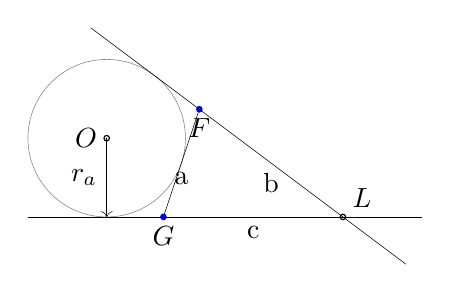
\begin{tikzpicture}[scale=1]
\tkzDefPoints{0/0/O, 0/-1/E, 3/-1/L}
\tkzDrawPoints(O,L)
\tkzDrawSegment[->](O,E)
\tkzLabelSegment[left](O,E){$r_a$}
\tkzLabelPoint[left](O){$O$}
\tkzLabelPoint[above right](L){$L$}
\tkzDrawCircle(O,E)
\tkzDefMidPoint(O,L)
\tkzGetPoint{C}
%\tkzDrawPoint(C)
%\tkzDrawCircle[dashed](C,O)
\tkzInterCC(O,E)(C,O)
\tkzGetPoints{A}{B}
%\tkzDrawPoints[color=red](A,B)
\tkzInterLC(O,L)(O,E) \tkzGetSecondPoint{D}
%\tkzDrawPoint[color=blue](D)
\tkzDefPointWith[orthogonal](D,O)  \tkzGetPoint{i}
 %\tkzDrawLines[add = 1 and 1,color=orange](D,i)
 \tkzInterLL(D,i)(A,L) \tkzGetPoint{F}
 \tkzInterLL(D,i)(B,L) \tkzGetPoint{G}
 \tkzDrawPoints[color=blue](F,G)
 \tkzDrawSegment(F,G)
 \tkzLabelSegment(F,G){a}
 \tkzLabelSegment(F,L){b}
 \tkzLabelSegment[below](G,L){c}
 \tkzLabelPoints(F,G)

%\tkzLabelPoint[color=red, above](A){$A$}
%\tkzLabelPoint[color=red, below](B){$B$}

\tkzDrawLines[add = 1/3 and 1/3](A,L B,L)
\end{tikzpicture}

\caption{Ex-radio $r_a$}
   
\end{figure}

Sea el triángulo $\triangle ABC$ de lados a,b y c, además de: $p=\frac{a+b+c}{2}$\\
Los ex-radios relativos a los lados a,b y c están dados por:
%formulas
$$ r_a=p\tan(\frac{A}{2}) $$
$$ r_b=p\tan(\frac{B}{2}) $$
$$ r_c=p\tan(\frac{C}{2}) $$

\newpage
%*********************
% EJERCICIO
\section{Teorema de áreas}

\begin{figure}[h]
\centering 
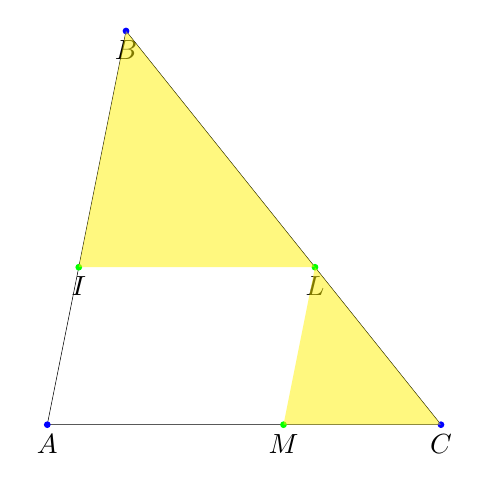
\begin{tikzpicture}[scale=1]
\tkzDefPoints{0/0/A, 1/5/B, 5/0/C}
\tkzDrawPolygon(A,B,C)
\tkzDrawPoints[color=blue](A,B,C)
\tkzLabelPoints(A,B,C)
\tkzDefBarycentricPoint(A=3,B=2) \tkzGetPoint{I}
\tkzDefBarycentricPoint(C=3,B=2) \tkzGetPoint{L}
\tkzDefLine[parallel=through L](A,I) \tkzGetPoint{i}
\tkzInterLL(A,C)(L,i) \tkzGetPoint{M}
\tkzLabelPoints(I,L,M)
\tkzDrawPoints[color=green](I,L,M)

 \tkzFillPolygon[color=yellow, opacity=.5 ](B,I,L)


\tkzFillPolygon[color=yellow, opacity=.5](M,L,C)
\end{tikzpicture}

\caption{Relación entre áreas}
   
\end{figure}
Sean $S, S_1, S_2$ áreas de las regiones triangulares $\triangle ABC$, $\triangle IBL$ y $\triangle MLC$ respectivamente.\\
Si $ABCD$ es un paralelogramo.\\
Entonces: 
%formulas
$$ S=(\sqrt{S_1}+\sqrt{S_2})^2 $$




\newpage

\section{\enquote{Le Monde} version}

\begin{tkzexample}[small]
\begin{tikzpicture}[scale=1.25]
  \tkzDefPoint(0,0){A}
  \tkzDefPoint(3,0){B}
  \tkzDefPoint(9,0){C}
  \tkzDefPoint(1.5,2){X}
  \tkzDefPoint(6,4){Y}
  \tkzDefCircle[circum](X,Y,B)       \tkzGetPoint{O}
  \tkzDefMidPoint(X,Y)               \tkzGetPoint{I}
  \tkzDefPointWith[orthogonal](I,Y)  \tkzGetPoint{i}
  \tkzDrawLines[add = 2 and 1,color=orange](I,i)
  \tkzInterLL(I,i)(A,B)              \tkzGetPoint{Z}
  \tkzInterLC(I,i)(O,B)              \tkzGetSecondPoint{M}
  \tkzDefPointWith[orthogonal](B,Z)  \tkzGetPoint{b}
  \tkzDrawCircle(O,B)
  \tkzDrawLines[add = 0 and 2,color=orange](B,b)
  \tkzDrawSegments(A,X B,X B,Y C,Y A,C X,Y)
  \tkzDrawSegments[color=red](X,Z Y,Z)
  \tkzDrawPoints(A,B,C,X,Y,Z,M,I)
  \tkzLabelPoints(A,B,C,Z)
  \tkzLabelPoints[above right](X,Y,M,I)
\end{tikzpicture}
\end{tkzexample}


\newpage
%*********************
% EJERCICIO
\section{Teorema de Pappus}

\begin{figure}[h]
\centering 
\begin{tikzpicture}[scale=1]
\tkzDefPoints{0/0/O, 0/-3/E, 6/-3/L}
\tkzDrawPoints(O,L)
\tkzLabelPoint[left](O){$O$}
\tkzLabelPoint[above right](L){$L$}
\tkzDrawCircle(O,E)
\tkzDefMidPoint(O,L)
\tkzGetPoint{C}
\tkzInterCC(O,E)(C,O)
\tkzGetPoints{A}{B}
\tkzDrawPoints[color=red](A,B)
\tkzLabelPoints(A,B){A,B}
\tkzDrawSegment(A,B)

\tkzDefPoint({-sqrt(35)/2},0.5){P}
\tkzDrawPoint[left](P)

\tkzDefPointBy[projection=onto A--B](P) \tkzGetPoint{M}
\tkzDrawPoint(M)
\tkzDrawSegment(P,M)
\tkzLabelSegment[below](P,M){x}

\tkzDefPointBy[projection=onto L--A](P) \tkzGetPoint{G}
\tkzDrawPoint(G)
\tkzDrawSegment(P,G)
\tkzLabelSegment[above](P,G){b}
\tkzDefPointBy[projection=onto L--B](P) \tkzGetPoint{H}
\tkzDrawPoint(H)
\tkzDrawSegment(P,H)
\tkzLabelSegment[left](P,H){a}
\tkzMarkRightAngles[fill=brown!20](A,G,P B,H,P B,M,P)
\tkzDrawSegment(A,G)
\tkzDrawSegment(B,H)
\end{tikzpicture}  
\caption{}
\end{figure}
Entonces:
$$x = \sqrt{ab}$$


\newpage
%*********************
% EJERCICIO
\section{Teorema}

\begin{figure}[h]
\centering 
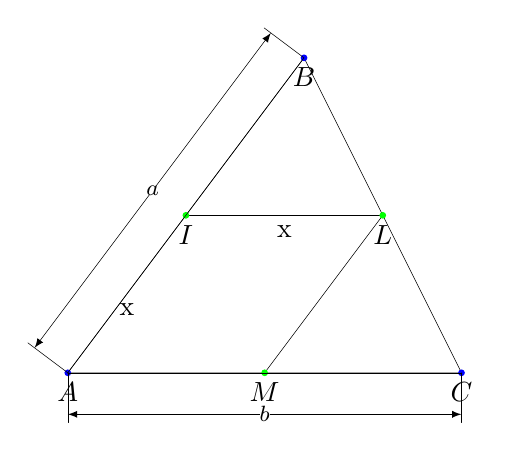
\begin{tikzpicture}[scale=1]
\tkzDefPoints{0/0/A, 3/4/B, 5/0/C}
\tkzDrawPolygon(A,B,C)
\tkzDrawPoints[color=blue](A,B,C)
\tkzLabelPoints(A,B,C)
\tkzDefMidPoint(A,B)\tkzGetPoint{I}
\tkzDefMidPoint(C,B)\tkzGetPoint{L}
\tkzDefLine[parallel=through L](A,I) \tkzGetPoint{i}
\tkzInterLL(A,C)(L,i) \tkzGetPoint{M}
\tkzLabelPoints(I,L,M)
\tkzDrawSegment(I,L)
\tkzDrawSegment(M,L)
\tkzLabelSegment(A,I){x}
\tkzLabelSegment(I,L){x}
\tkzDrawPoints[color=green](I,L,M)
\tkzDrawSegment[dim={$a$,15pt,}](A,B)
\tkzDrawSegment[dim={$b$,-15pt,}](A,C)
\end{tikzpicture}
\caption{}
\end{figure}
Entonces: 
%formulas
$$ x=\frac{ab}{a+b} $$


\newpage
%*********************
% EJERCICIO
\section{Teorema de Pappus}

\begin{figure}[h]
\centering 
\begin{tikzpicture}[scale=1]
\tkzDefPoints{0/0/O, 0/-3/E, 6/-3/L}
\tkzDrawPoints(O,L)
\tkzLabelPoint[left](O){$O$}
\tkzLabelPoint[above right](L){$L$}
\tkzDrawCircle(O,E)
\tkzDefMidPoint(O,L)
\tkzGetPoint{C}
\tkzInterCC(O,E)(C,O)
\tkzGetPoints{A}{B}
\tkzDrawPoints[color=red](A,B)
\tkzLabelPoints(A,B){A,B}
\tkzDrawSegment(A,B)

\tkzDefPoint({-sqrt(35)/2},0.5){P}
\tkzDrawPoint[left](P)

\tkzDefPointBy[projection=onto A--B](P) \tkzGetPoint{M}
\tkzDrawPoint(M)
\tkzDrawSegment(P,M)
\tkzLabelSegment[below](P,M){x}

\tkzDefPointBy[projection=onto L--A](P) \tkzGetPoint{G}
\tkzDrawPoint(G)
\tkzDrawSegment(P,G)
\tkzLabelSegment[above](P,G){b}
\tkzDefPointBy[projection=onto L--B](P) \tkzGetPoint{H}
\tkzDrawPoint(H)
\tkzDrawSegment(P,H)
\tkzLabelSegment[left](P,H){a}
\tkzMarkRightAngles[fill=brown!20](A,G,P B,H,P B,M,P)
\tkzDrawSegment(A,G)
\tkzDrawSegment(B,H)
\end{tikzpicture}  
\caption{}
\end{figure}
Entonces:
$$x = \sqrt{ab}$$


\newpage
%*********************
% EJERCICIO
\section{Teorema trapecio}

\begin{figure}[h]
\centering 
\begin{tikzpicture}[scale=1]
\tkzDefPoints{-3/0/A, 0/4/B, 2/4/C, 7/0/D}
\tkzDrawPolygon(A,B,C,D)
\tkzDrawPoints[color=purple](A,B,C,D)
\tkzLabelPoints(A,B,C,D)
\tkzDefMidPoint(B,C)\tkzGetPoint{I}
\tkzDefMidPoint(A,D)\tkzGetPoint{L}
\tkzDrawSegment(I,L)
\tkzLabelSegment(I,L){x}
\tkzDrawPoints[color=green](I,L)
\tkzDrawSegment[dim={$a$,-15pt,}](A,D)
\tkzDrawSegment[dim={$b$,10pt,}](B,C)
\tkzMarkAngle[size=0.3cm](D,A,B);
\tkzLabelAngle[pos=-.6](B,A,D){$\alpha$}
\tkzMarkAngle[size=0.3cm](C,D,A);
\tkzLabelAngle[pos=-.6](A,D,C){$\beta$}
\tkzMarkSegments[mark = *, size=1.5](B,I I,C)
\tkzMarkSegments[mark = ||, size=3](A,L L,D)
\end{tikzpicture}
\caption{}
\end{figure}
Sea el trapecio $ABCD$. Si $\alpha+\beta=90^{\circ}$\\
Entonces:
%formulas
$$ x=\frac{a-b}{2} $$


\newpage
%*********************
% EJERCICIO
\section{Teorema triángulo trpecio}

\begin{figure}[h]
\centering 
\begin{tikzpicture}[scale=1]
\tkzDefPoints{-2/0/A, 0/4/B, 4/0/C}
\tkzDrawPolygon(A,B,C)
\tkzDrawPoints[color=red](A,B,C)
\tkzLabelPoints(A,B,C)
%\tkzDrawSegment[dim={$a$,-15pt,}](A,D)
\tkzDefPoints{-3/0/M, 6/0/N}
\tkzDrawSegments(A,M C,N)
\tkzDefLine[bisector,normed](B,A,M) \tkzGetPoint{a}
%\tkzShowLine[bisector,gap=4,size=2,color=red](B,A,M)
\tkzDrawLines[new,dashed,add= 0 and 3](A,a)

\tkzDefPointBy[projection=onto A--a](B) \tkzGetPoint{F}
\tkzDrawSegments(B,F A,F)
\tkzMarkRightAngle[fill=orange!10,opacity=.4](A,F,B)
\tkzMarkAngle[size=0.3cm](B,A,F);
\tkzLabelAngle[pos=.6](B,A,F){$\theta$}
\tkzMarkAngle[size=0.3cm](F,A,M);
\tkzLabelAngle[pos=.6](F,A,M){$\theta$}

\tkzDefLine[bisector,normed](N,C,B) \tkzGetPoint{c}
\tkzDrawLines[new,dashed,add= 0 and 3](C,c)
\tkzDefPointBy[projection=onto C--c](B) \tkzGetPoint{G}
\tkzDrawSegments(B,G C,G)
\tkzMarkRightAngle[fill=orange!10,opacity=.4](B,G,C)
\tkzMarkAngle[size=0.3cm](G,C,B);
\tkzLabelAngle[pos=.6](G,C,B){$\beta$}
\tkzMarkAngle[size=0.3cm](N,C,G);
\tkzLabelAngle[pos=.6](N,C,G){$\beta$}

\tkzDrawSegment[dim={$x$,0pt,}](F,G)
\tkzLabelSegment[left, above, color=red](A,B){a}
\tkzLabelSegment[right, above, color=red](C,B){b}
\tkzLabelSegment[below, color=red](A,C){c}

\end{tikzpicture}
\caption{}
\end{figure}
Sea el triángulo $\triangle ABC$ de lados $a,b y c$.\\ 
Se cumple:
%formulas
$$ x=\frac{a+b+c}{2} $$

\newpage

%*********************
% EJERCICIO
\section{Teorema de Visscher}

\begin{figure}[h]
    \centering
\begin{tikzpicture}
\tkzDefPoints{-3/0/A, 0/(sqrt{27})/B,3/0/C,0/(sqrt{3})/P}
\tkzDrawPolygon(A,B,C)
\tkzDrawPoint(P)
\tkzLabelPoints(A,B,C,P)
\tkzDrawSegments[gray, dotted, thick](B,P A,P P,C)

\tkzMarkAngles[size=0.2cm](C,P,B B,P,A A,P,C);
\tkzLabelAngles[pos=.4](C,P,B B,P,A A,P,C){$\theta$}

\tkzLabelSegments(A,P){x}
\tkzLabelSegments(P,B){y}
\tkzLabelSegments(P,C){z}
\end{tikzpicture}  
\caption{Triángulo}
\end{figure}
Sea el $\triangle ABC$ y $P$ es un punto interior de su región interior.  
Si $(x+y+z)$ es mínimo.\\
Entonces:
$$ m\angle APB=m\angle BPC= m\angle APC= \theta=120^{\circ}$$
$$P: punto de Fermat$$

\newpage

%*********************
% EJERCICIO
\section{Ángulo entre rectas}

\begin{figure}[h]
    \centering
\begin{tikzpicture}
\tkzInit[xmax=11, ymax=8]
\tkzDrawX \tkzDrawY
\tkzClip[space=-1]
\tkzDefPoints{1/1/A,2/6/B,9/6/C,9/1/D}
\tkzDrawSegments[<->](A,C B,D)
\coordinate (E) at (intersection of A--C and B--D);
\tkzMarkAngle[size=0.5cm](C,E,B);
\tkzLabelAngle[pos=.8](C,E,B){$\theta$}
\tkzLabelSegment[rotate=33](A,C){$A_1x+B_1y+C_1=0$}
\tkzLabelSegment[rotate=-35](B,D){$A_2x+B_2y+C_2=0$}

\end{tikzpicture}  
\caption{}
\end{figure}
Dadas las ecuaciones de las rectas: $A_1x+B_1y+C_1=0$ y $A_2x+B_2y+C_2=0$.\\
El ángulo $\theta$ determinado por la intersección de las rectas, está dado por
$$ \theta=\arctan(\frac{A_1B_2-A_2B_1}{A_1A_2+B_1B_2})$$


\newpage

%*********************
% EJERCICIO
\section{Teorema de tangencia}

\begin{figure}[h]
    \centering
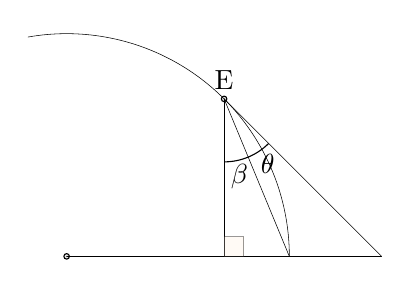
\begin{tikzpicture}
\tkzDefPoints{0/0/D,2/2/E,4/0/F,sqrt(8)/0/R}
\tkzDrawPoints(D,E)
\tkzLabelPoint[above](E){E}
\tkzDefPointBy[projection=onto D--R](E) \tkzGetPoint{T}
\tkzDrawSegments(D,F E,F E,R E,T)
\tkzDrawArc[angles](D,E)(0,100)
\tkzMarkRightAngle[fill=orange!10,opacity=.4](E,T,R)
\tkzMarkAngle[size=0.8](R,E,F)
\tkzLabelAngle(R,E,F){$\theta$}
\tkzMarkAngle[size=0.8](T,E,R)
\tkzLabelAngle(T,E,R){$\beta$}

\end{tikzpicture}  
\caption{Triángulo}
\end{figure}
Si $E$ es un punto de tangencia. \\
Entonces:
$$ \theta=\beta$$


\newpage
%*********************
% EJERCICIO
\section{Punto de tangencia}

\begin{figure}[h]
\centering 
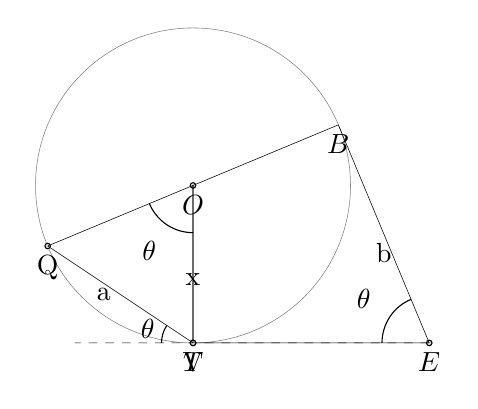
\begin{tikzpicture}[scale=1]
\tkzDefPoints{0/0/O, 0/-2/T, 3/-2/E}
\tkzDrawPoints(O,E,T)
\tkzLabelPoints(O,E,T){O,E,T}
\tkzDefMidPoint(O,E)
\tkzGetPoint{G}
%\tkzDrawCircle(G,O)
\tkzDrawCircle(O,T)
\tkzInterCC(G,O)(O,T)
\tkzGetSecondPoint{B}
\tkzLabelPoints(B){B}
\tkzDrawPolygon(O,T,E,B)
%\tkzDrawLines[add=0 and 2.2,dashed](B,O E,T)
\tkzInterLC(B,O)(O,T)
\tkzGetSecondPoint{Q}
\tkzDrawPoint(Q)
\tkzLabelPoint(Q){Q}
%SEGUNDO CIRCULO
\tkzInterCC(O,Q)(Q,O)
\tkzGetFirstPoint{H}
\tkzGetSecondPoint{J}

\tkzInterCC(O,T)(T,O)
\tkzGetFirstPoint{K}
\tkzGetSecondPoint{L}

%Centro
\tkzInterLL(H,J)(K,L)
\tkzGetPoint{I}
%\tkzDrawPoints[color=red](I)
%\tkzLabelPoint[color=red,above,left](I){I}
%C\’{\i}rculo
%\tkzDrawCircle[thick](I,O)

\tkzInterLC(E,T)(I,O)
\tkzGetSecondPoint{V}
\tkzDrawPoint(V)
\tkzLabelPoint(V){V}

\tkzDrawLine[add=0 and 1/2,dashed](E,V)
\tkzDrawPolygon(V,T,O,Q)

\tkzMarkAngle[size=0.6](B,E,T)
\tkzLabelAngle(B,E,T){$\theta$}
\tkzMarkAngle[size=0.6](Q,O,T)
\tkzLabelAngle(Q,O,T){$\theta$}
\tkzDefPointBy[projection=onto E--V](Q) \tkzGetPoint{S}
\tkzMarkAngle[size=0.4](Q,V,S)
\tkzLabelAngle[pos=0.6pt](Q,V,S){$\theta$}

\tkzLabelSegments(B,E){b}
\tkzLabelSegments(O,T){x}
\tkzLabelSegments[left](Q,V){a}

\end{tikzpicture}  
\caption{}
\end{figure}
Si $T$ es punto de tangencia.\\
Entonces:
$$x = \sqrt{ab}$$

\newpage
%*********************
% EJERCICIO
\section{Corolario}

\begin{figure}[h]
\centering 
\begin{tikzpicture}[scale=1]
\tkzDefPoints{0/0/A, 2/5/B, 5/0/C}
\tkzDrawPolygon(A,B,C)
\tkzDrawPoints[color=blue](A,B,C)
\tkzLabelPoints(A,C)
\tkzLabelPoints[above](B)
\tkzOrthoCenter(A,C,B) \tkzGetPoint{Y}
\tkzDrawPoints[color=blue](Y,G)
\tkzCircumCenter(A,B,C) \tkzGetPoint{G}
\tkzLabelPoints[below](Y,G)
\tkzDrawSegments(B,Y B,G)
\tkzMarkAngle[size=0.6](A,B,C)
\tkzLabelAngle(A,B,C){$60^{\circ}$}
\end{tikzpicture}

\caption{}
   
\end{figure}
Sea el triángulo $\triangle ABC$, de ortocentro $Y$ y circuncentro $G$.\\
Si $m\angle ABC=60^{\circ}$. Entonces:
%formulas
$$ \overline{BY}=\overline{BG} $$


\newpage
%*********************
% EJERCICIO
\section{Propiedad triángulo}

\begin{figure}[h]
\centering 
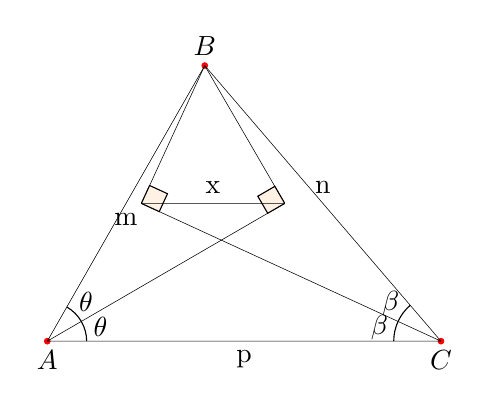
\begin{tikzpicture}[scale=1]
\tkzDefPoints{-2/0/A, 0/3.5/B, 3/0/C}
\tkzDrawPoints[color=red](A,B,C)
\tkzLabelPoints(A,C)
\tkzLabelPoints[above](B)
\tkzDrawPolygon(A,B,C)
\tkzLabelSegments(A,B){m}
\tkzLabelSegments[above](C,B){n}
\tkzLabelSegments[below](A,C){p}

\tkzDefLine[bisector,normed](B,A,C) \tkzGetPoint{a}
\tkzDefPointBy[projection=onto A--a](B) \tkzGetPoint{F}
\tkzDrawSegments(B,F A,F)
\tkzMarkRightAngle[fill=orange!10](B,F,A)
\tkzMarkAngle[size=0.5cm](F,A,B)
\tkzLabelAngle[pos=.7](F,A,B){$\theta$}
\tkzMarkAngle[size=0.5cm](C,A,F)
\tkzLabelAngle[pos=.7](C,A,F){$\theta$}

\tkzDefLine[bisector,normed](B,C,A) \tkzGetPoint{d}
\tkzDefPointBy[projection=onto C--d](B) \tkzGetPoint{W}
\tkzDrawSegments(B,W C,W)
\tkzMarkRightAngle[fill=orange!10](B,W,C)
\tkzMarkAngle[size=0.6cm](B,C,W)
\tkzLabelAngle[pos=.8](B,C,W){$\beta$}
\tkzMarkAngle[size=0.6cm](W,C,A)
\tkzLabelAngle[pos=.8](W,C,A){$\beta$}

\tkzDrawSegment(F,W)
\tkzLabelSegment[above](F,W){x}
\end{tikzpicture}
\caption{}
\end{figure}
Sea el triángulo $\triangle ABC$ \\ 
Se cumple:
%formulas
$$ x=\frac{m+n-p}{2} $$

\newpage

%*********************
% EJERCICIO

\section{Teoremas de triángulos}
\subsection{Teorema incentro baricentro}

\begin{figure}[h]
\centering 
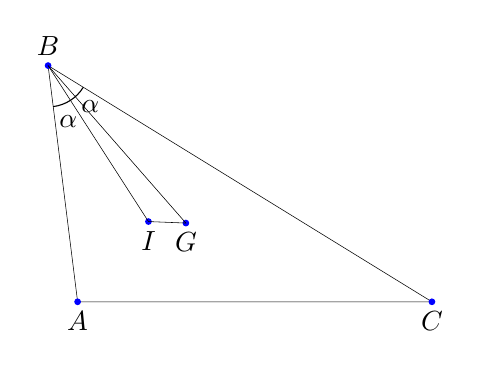
\begin{tikzpicture}[scale=0.75]
\tkzDefPoints{-3/0/A, -3.5/4/B, 3/0/C}
\tkzDrawPolygon(A,B,C)
\tkzDrawPoints[color=blue](A,B,C)
\tkzLabelPoints(A,C)
\tkzLabelPoints[above](B)
\tkzInCenter(A,B,C) \tkzGetPoint{I}
\tkzCentroid(A,B,C) \tkzGetPoint{G}
\tkzDrawPoints[color=blue](I,G)
\tkzLabelPoints[below](I,G)
\tkzDrawSegments(B,I B,G I,G)
\tkzMarkAngle[size=0.7](A,B,I)
\tkzLabelAngle(A,B,I){$\alpha$}
\tkzMarkAngle[size=0.7](I,B,C)
\tkzLabelAngle(I,B,C){$\alpha$}
\end{tikzpicture}

\caption{}
   
\end{figure}
Sea el triángulo $\triangle ABC$, de incentro $I$ y baricentro $G$.\\
Si $\overline{IG} \parallel  \overline{AC}$. Entonces:
%formulas
$$ AC = \frac{AB+BC}{2} $$


%*********************
% EJERCICIO
\subsection{Teorema de área y bisectriz interior}

\begin{figure}[h]
\centering 
\begin{tikzpicture}[scale=1]
\tkzDefPoints{0/0/A, 1/3/B, 5/0/C}
\tkzDrawPolygon(A,B,C)
\tkzDrawPoints[color=blue](A,B,C)
\tkzLabelPoints(A,C){A,C}
\tkzLabelPoints[above](B){B}
\tkzDrawBisector(A,B,C) \tkzGetPoint{D}
\tkzLabelPoints(D){D}
\tkzFillPolygon[color=yellow, opacity=.5 ](A,B,D)
\tkzFillPolygon[color=green, opacity=.5](D,B,C)
\tkzMarkAngle[size=0.7](A,B,D)
\tkzLabelAngle(A,B,D){$\alpha$}
\tkzMarkAngle[size=0.7](D,B,C)
\tkzLabelAngle(D,B,C){$\alpha$}

\tkzCentroid(A,B,D) \tkzGetPoint{M}
\tkzLabelPoint(M){$S_1$}
\tkzCentroid(D,B,C) \tkzGetPoint{N}
\tkzLabelPoint(N){$S_2$}

\tkzLabelSegment[below](A,D){m}
\tkzLabelSegment[below](D,C){n}
\end{tikzpicture}

\caption{}
   
\end{figure}
Si $\overline{BD}$ es bisectriz interior del triángulo $\triangle ABC$\\
Entonces: 
%formulas
$$ \frac{S_1}{S_2}=\frac{a}{b}=\frac{m}{n} $$

\newpage
%*********************
% EJERCICIO
\subsection{Teorema de Van Aubel}
\begin{figure}[h]
\centering 
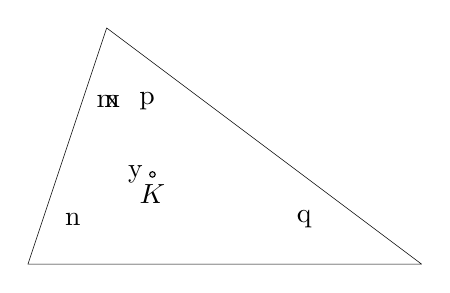
\begin{tikzpicture}[scale=1]
\tkzDefPoints{0/0/A, 1/3/B, 5/0/C}
\tkzInCenter(A,B,C) \tkzGetPoint{J}
\tkzDrawPolygon(A,B,C)

\tkzDrawBisector(A,B,C) \tkzGetPoint{D}
\tkzDrawBisector(A,C,B) \tkzGetPoint{E}
\tkzDrawBisector(C,A,B) \tkzGetPoint{F}
\tkzInterLL(B,D)(C,E) \tkzGetPoint{K}
\tkzDrawPoint(K)
\tkzLabelPoint(K){$K$}

\tkzLabelSegment[left](B,E){m}
\tkzLabelSegment[left](E,A){n}
\tkzLabelSegment[left](B,K){x}
\tkzLabelSegment[left](K,D){y}
\tkzLabelSegment[right](B,F){p}
\tkzLabelSegment[right](F,C){q}
\end{tikzpicture}

\caption{}
   
\end{figure}
Sea $K$ el punto de intersección de las cevianas de un triángulo.\\
Se cumple: 
%formulas
$$ \frac{x}{y}=\frac{m}{n}=\frac{p}{q} $$

%*********************
% EJERCICIO
\subsection{Teorema de raíces de áreas triangulares}
\begin{figure}[h]
\centering 
\begin{tikzpicture}[scale=1]
\tkzDefPoints{0/0/A, 2/5/B, 5/0/C}
\tkzDrawPolygon(A,B,C)
\tkzDrawCircle[in](A,B,C) \tkzGetPoint{I}
\tkzDrawPoints(A,B,C)
\tkzDefPointBy[projection=onto A--C](I) \tkzGetPoint{M}
\tkzDrawPoint(M)
\tkzInterLC(A,I)(I,M) \tkzGetFirstPoint{E}
\tkzInterLC(B,I)(I,M) \tkzGetFirstPoint{R}
\tkzInterLC(C,I)(I,M) \tkzGetFirstPoint{T}

\tkzDefTangent[at=E](I) \tkzGetPoint{e}
\tkzInterLL(E,e)(A,B) \tkzGetPoint{J}
\tkzInterLL(E,e)(A,C) \tkzGetPoint{N}
\tkzDrawSegment(J,N)
\tkzDefTangent[at=R](I) \tkzGetPoint{r}
\tkzInterLL(R,r)(B,A) \tkzGetPoint{K}
\tkzInterLL(R,r)(B,C) \tkzGetPoint{M}
\tkzDrawSegment(K,M)
\tkzDefTangent[at=T](I) \tkzGetPoint{t}
\tkzInterLL(T,t)(C,B) \tkzGetPoint{P}
\tkzInterLL(T,t)(C,A) \tkzGetPoint{O}
\tkzDrawSegment(P,O)

\tkzFillPolygon[color=yellow, opacity=.5 ](A,J,N)
\tkzFillPolygon[color=green, opacity=.5](B,K,M)
\tkzFillPolygon[color=red, opacity=.5](C,P,O)

\tkzInCenter(A,J,N) \tkzGetPoint{Y}
\tkzLabelPoint(Y){$A_1$}
\tkzInCenter(B,K,M) \tkzGetPoint{U}
\tkzLabelPoint(U){$A_2$}
\tkzInCenter(C,P,O) \tkzGetPoint{H}
\tkzLabelPoint(H){$A_3$}


\end{tikzpicture}

\caption{}
   
\end{figure}
Si $A$ es el área de la región triangular $\triangle ABC$. Entonces: 
%formulas
$$ \sqrt{A}=\sqrt{A_1}+\sqrt{A_2}+\sqrt{A_3} $$

\newpage
%*********************
% EJERCICIO
\section{Propiedades de  triángulos}

\subsection{Propiedades de altura de ángulo doble en ángulo triple}
\begin{figure}[h]
\centering 
\begin{tikzpicture}[scale=2 ]
\tkzDefPoint(0,0){A}
\tkzDefPoint(5,0){B}
\tkzDefTriangle[two angles = 60 and 30](A,B) \tkzGetPoint{C}
\tkzDrawSegment(A,B)
\tkzDrawPoints(A,B)
\tkzLabelPoints(A,B)
\tkzDrawSegments(A,C B,C)
\tkzDrawPoints(C)
\tkzLabelPoints[above](C)
\tkzDefTriangle[two angles = 90 and 20](C,A) \tkzGetPoint{D}
\tkzDrawSegment(A,D)
\tkzDefPointBy[projection=onto A--D](C) \tkzGetPoint{F}
\tkzDefPointBy[projection=onto A--B](D) \tkzGetPoint{G}
\tkzDrawSegments(C,F D,G)
\tkzLabelSegment[below](C,F){k}
\tkzLabelSegment(D,G){x}
\tkzLabelAngle[pos=.6](D,A,C){$\theta$}
\tkzLabelAngle[pos=.6](B,A,D){$2\theta$}
\tkzMarkRightAngles[size=.15,fill=gray!15](C,F,D A,C,B D,G,B)

\end{tikzpicture}
\caption{}
\end{figure}
% ======
Sea el triángulo rectangulo $\angle ABC$. \\
Se cumple: 
%formulas
$$ x = 2k $$



\newpage
%*********************
% EJERCICIO
\section{Teoremas cuadriláteros}
\subsection{Bisectrices de trapecio}

\begin{figure}[h]
\centering
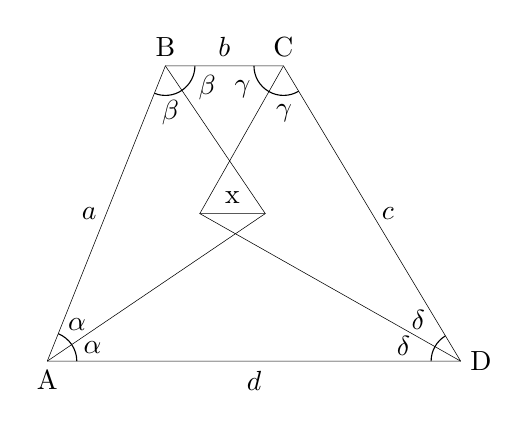
\begin{tikzpicture}[scale=0.75]
\tkzDefPoints{0/0/A,2/5/B,4/5/C,7/0/D}
\tkzDrawPolygon(A,B,C,D)
\node[below] at(A) {A};
\node[above] at(B) {B};
\node[above] at(C) {C};
\node[right] at(D) {D};

\tkzDefLine[bisector,normed](D,A,B) \tkzGetPoint{a}
\tkzDefLine[bisector,normed](A,B,C) \tkzGetPoint{b}
\tkzInterLL(A,a)(B,b) \tkzGetPoint{M}
\tkzDrawSegments(A,M B,M)

\tkzDefLine[bisector,normed](B,C,D) \tkzGetPoint{c}
\tkzDefLine[bisector,normed](C,D,A) \tkzGetPoint{d}
\tkzInterLL(D,d)(C,c) \tkzGetPoint{N}
\tkzDrawSegments(C,N D,N M,N)
\tkzLabelSegment[above](M,N){x}
\tkzLabelSegment[left](A,B){$a$}
\tkzLabelSegment[above](B,C){$b$}
\tkzLabelSegment[right](C,D){$c$}
\tkzLabelSegment[below](D,A){$d$}

\tkzMarkAngle[size=0.5cm](D,A,M)
\tkzMarkAngle[size=0.5cm](M,A,B)
\tkzMarkAngle[size=0.5cm](A,B,M)
\tkzMarkAngle[size=0.5cm](M,B,C)
\tkzMarkAngle[size=0.5cm](B,C,N)
\tkzMarkAngle[size=0.5cm](N,C,D)
\tkzMarkAngle[size=0.5cm](C,D,N)
\tkzMarkAngle[size=0.5cm](N,D,A)

\tkzLabelAngle[pos=.8](D,A,M){$\alpha$}
\tkzLabelAngle[pos=.8](M,A,B){$\alpha$}
\tkzLabelAngle[pos=.8](A,B,M){$\beta$}
\tkzLabelAngle[pos=.8](M,B,C){$\beta$}
\tkzLabelAngle[pos=.8](B,C,N){$\gamma$}
\tkzLabelAngle[pos=.8](N,C,D){$\gamma$}
\tkzLabelAngle[pos=1](C,D,N){$\delta$}
\tkzLabelAngle[pos=1](N,D,A){$\delta$}

\end{tikzpicture}  
\caption{}
\end{figure}

Sea el trapecio $ABCD$\\
Se cumple:
%formula
$$ x = \frac{(a+c)-(b+d)}{2} $$

%*********************
% EJERCICIO
\subsection{Teorema diagonales perpendiculares}

\begin{figure}[h]
\centering
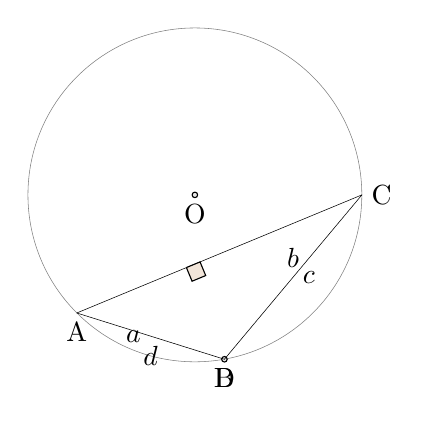
\begin{tikzpicture}[scale=0.75]
\tkzDefPoints{0/0/A,{2+sqrt{8}}/2/C,2.5/{2-sqrt{31}/2}/D,2/2/O}
\tkzDrawCircle(O,A)
\tkzDrawPoint(O)
\tkzLabelPoint(O){O}
\node[below] at(A) {A};
%\node[above] at(B) {B};
\node[right] at(C) {C};
\node[below] at(D) {D};
\tkzDefPointBy[projection=onto A--C](D) \tkzGetPoint{M}
\tkzInterLC(D,M)(O,A) \tkzGetSecondPoint{B}
\tkzDrawPoint(B)
\tkzLabelPoint(B){B}
\tkzDrawPolygon(A,B,C,D)
\tkzLabelSegment[left](A,B){$a$}
\tkzLabelSegment[above](B,C){$b$}
\tkzLabelSegment[right](C,D){$c$}
\tkzLabelSegment[below](D,A){$d$}
\tkzDrawSegments(A,C B,D)
\tkzMarkRightAngles[fill=brown!20](C,M,B)

\end{tikzpicture}  
\caption{}
\end{figure}

Sea el cuadrilátero $ABCD$ cuyas deiagonales se intersectan en forma perpendicular\\
Se cumple:
%formula
$$ a^2+b^2=c^2+d^2 $$



\newpage
\section{Aritmética}
\begin{multicols}{2}
\subsection{Teorema de Wilson}
Si P es un número primo entonces:
$$ (P-1)! = \overset{\circ}{P} - 1 $$
\underline{Ejemplo:}\\
11 es un número primo, entonces:
\begin{equation*}
\begin{split}
10! &= 1\cdot2\cdot3\cdot4\cdot5\cdot6\cdot7\cdot8\cdot9\cdot10 \\
10! &= 3628800\\
10! &= \overset{\circ}{11} - 1
\end{split}
\end{equation*}


\end{multicols}

%
\section{Cálculo}
\subsection{Teoría}
\subsubsection{Longitud de arco en coordenadas cartesianas}


%%%%%%%%%%%%%%%%%%%%%%%
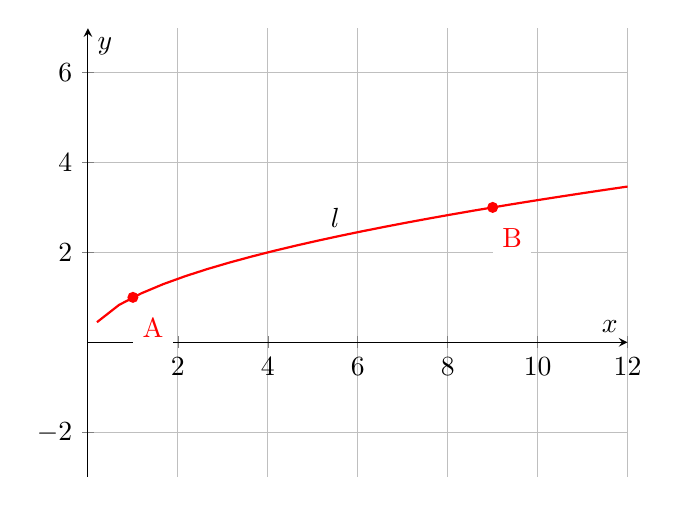
\begin{tikzpicture}
\begin{axis}[axis lines=middle,axis equal, grid=both, xlabel=$x$,    ylabel=$y$,domain=0.2:12, xmax=12,xmin=0,ymax=4,ymin=0]
\addplot[red,thick] {( x^(0.5)};
\fill[red] (1,1) circle (2pt) node [below right,fill=white,yshift=-4pt] {A};


\fill[red] (9,3) circle (2pt) node [below right,fill=white,yshift=-4pt] {B};
\draw[thick,red] (5.5,2.3453) coordinate (a) ;
\draw (a) node[above] {$l$};

\end{axis}
\end{tikzpicture}
\\Sea $f(x)$ una función continua y derivable.\\
La longitud de arco $l$, está dado por:
\begin{equation*}
l=\int_a^b\sqrt{1+{f'(x)}^2}
\mathrm{d}x=
\end{equation*}

\end{document}
